%****************figure: demo user-specific************************
\begin{figure}
\begin{center}
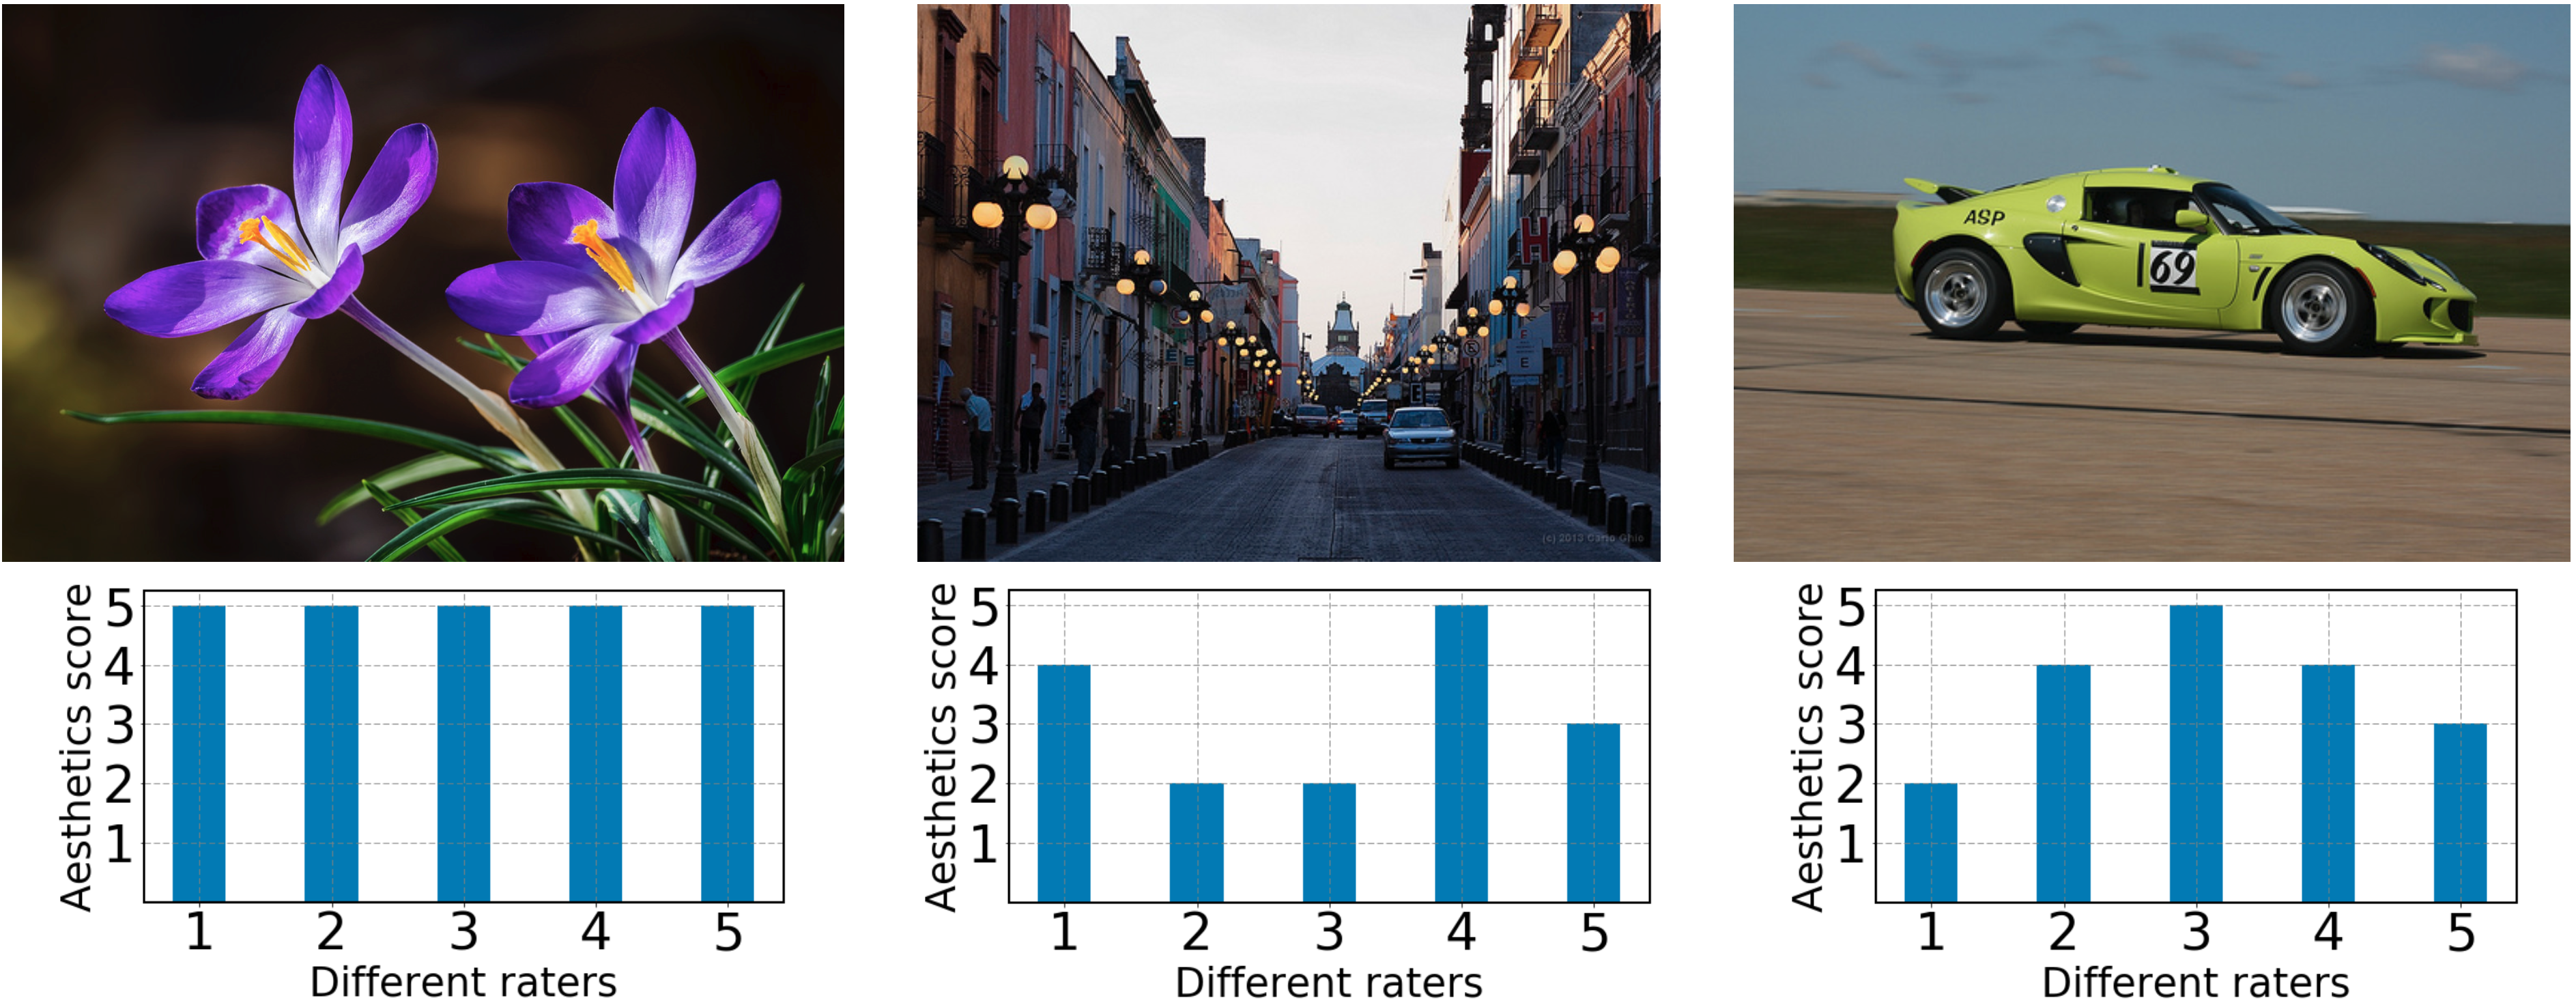
\includegraphics[width=1\columnwidth]{figures/demo1}
%\vspace{-0.3in}
\end{center}
\caption{Examples illustrating personal aesthetic preferences. Each image is rated by 5 different users. As can be seen, on the first example, ratings are consistent among the users while on the other two, different users manifest very different visual tastes. Individual users may have their unique preference with respect to visual attributes or contents of an image when they judge its aesthetic quality.} 
\label{demoImage}
\end{figure}
%****************************************************************

\section{Introduction}

Automatic assessment of image aesthetics is an important problem that has a variety of applications such as image search, creative recommendation, photo ranking and personal album curation, etc.~\cite{marchesotti2015discovering, lu2015deep}. It is a challenging task that requires high-level understanding of photographic attributes and semantics in an image. Only recently, there has been a significant progress due to the advancement in deep learning that can learn such high-level information effectively from data \cite{lu2014rapid, lu2015deep}. Although many successful deep learning-based approaches have been proposed for learning generic aesthetics classifiers, efforts on learning user-specific aesthetic models are quite limited. 

Image aesthetics rating is well known to be a highly subjective task as individual users have very different visual preferences. This has been observed in earlier rule-based photo ranking systems such as~\cite{yeh2010personalized, yeh2014personalized, vessel2014personalized}.  
For example, Figure~\ref{demoImage} shows example images and their aesthetic scores (1 to 5) rated by five different users following careful instructions. As can be seen, ratings for each image could vary significantly among the users. This is expected as different users may have very different opinions with respect to photographic attributes (composition, lighting, color) or semantic contents of the image (portrait, landscape, pets). Therefore, learning individual user's visual preference is a crucial next step in image aesthetics research.  

We refer to this problem as \textbf{personalized image aesthetics} and aim to address it by adapting a generic aesthetics model for individual user's preference. However, this is a challenging task as we typically need to learn such preference from a very limited set of annotated examples from each user. For example, in photo organization softwares, it is desired to minimize user's annotation effort. An effective strategy in such applications is to leverage active learning by automatically selecting representative images and suggest them to users for rating.

For investigating this problem with a learning-based approach, a labeled dataset with rater's identities are needed for training and evaluation purposes. Existing aesthetics datasets are not appropriate as they either do not have rater identities~\cite{murray2012ava} or are limited in size~\cite{kang2014convolutional}. Therefore, we introduce two new datasets specifically tailored for this task: (1) Flickr Images with Aesthetics Annotation Dataset (FLICKR-AES) which contains 40,000 Flickr images labeled by 210 unique Amazon Mechanical Turk (AMT)\footnote{https://www.mturk.com} annotators; (2) Real Album Curation Dataset (REAL-CUR) that contains 14 real user's photo albums with aesthetic scores provided by the album owners. 

To learn the average aesthetic preference of a typical user~\cite{bronstad2007beauty, kaplan1989experience}, we first use the relatively large FLICKR-AES dataset to train a powerful, generic aesthetics prediction model which performs competitively to the state of the art. Then, we present a novel approach for personalizing image aesthetics by adapting the generic model to individual users. To cope with a limited number of annotated examples from a user, we adopt a residual-based model adaptation scheme which is designed to learn a scalar offset to the generic aesthetic score for each user. 

Inspired by the studies~\cite{dhar2011high, luo2011content, murray2012ava} which leverage both aesthetic attributes and content information to improve the performance of generic aesthetics rating, we study feature representations effective for personalized aesthetics learning, and observed that features trained for generic aesthetics prediction, aesthetics attributes classification, and semantic content classification are all important for learning personalized image aesthetics models. We further show in experiments that our personalized aesthetics model with this combined feature representation significantly outperforms an existing collaborative filtering-based method.

Finally, we introduce an active personalized aesthetics learning algorithm for real-world application scenarios such as interactive photo album curation. Results demonstrate that our method compares favorably to typical active learning-based methods in the previous literature. 

Our main contributions are three-fold:
\begin{itemize}
\vspace{-0.1in}
  \item We address the problem of personalized image aesthetics, and introduce two new datasets to facilitate research in this direction.
  \vspace{-0.1in}
  \item We systematically analyze correlation between user ratings and image contents/attributes, and propose a novel approach for learning a personalized image aesthetics model with a residual-based model adaptation scheme.
  \vspace{-0.1in}
   \item We propose an active personalized image aesthetics learning algorithm for real-world image search and curation applications.
\end{itemize}

